\documentclass[11pt]{article}
\usepackage[spanish]{babel}
\usepackage[T1]{fontenc}
\usepackage{amsmath,amsfonts,amssymb,amsthm}
\usepackage{amsfonts}
\usepackage{graphicx}
\usepackage{geometry}
\usepackage{newpxtext,euler}
\usepackage{float}
\usepackage{xcolor}
\usepackage{geometry}
 \geometry{
 a4paper,
 total={170mm,245mm},
 left=20mm,
 top=30mm,
 }
\pagestyle{empty}

\title{Taller II}

\author{Bourbaki}
\date{\today}


\begin{document}

\maketitle

\begin{enumerate}
    \item Mostrar que si $e^z = e^w$ entonces existe un entero $k$ tal que $w = z + 2k\pi i$.\\

    \begin{proof}
    Supongamos que $e^z=e^w$, $z=a+bi$, $w=c+di$, entonces

    $$e^{a}e^{bi}=e^{c}e^{di},$$

    es claro que $|e^z|=|e^w|$ y por tanto $e^a=e^c$, por la inyectividad de la exponencial $a=c$, además $e^{bi}=e^{di}$, esto es

    $$\cos(b)+i\sin(b)=\cos(d)+i\sin(d),$$ 

    como estas ecuaciones determinan un único punto en la circúnferencia, entonces $(d-b)=2\pi k$, $k\in \mathbb{Z}$, por lo tanto

    \begin{align*}
      w-z&=c+di-a-bi\\
        &=a-a+i(d-b)\\
        &=i(2\pi k)
    ,\end{align*}

con $k\in \mathbb{Z}$

    \end{proof}

    \item Si $\theta$ es real, mostrar que
    \[
    \cos \theta = \frac{e^{i \theta} + e^{-i \theta}}{2}, \quad \sin \theta = \frac{e^{i \theta} - e^{-i \theta}}{2i}.
    \]

    \begin{proof}
    Pues lo que pasa es que eso es trivial allí, note que los numeradores son un complejo más su conjugado y un complejo menos su conjugado, entonces usted se acuerda que Pastrán dijo que eso daba 2 veces la parte real y 2i la parte imaginaria,  o sea

    $$\frac{e^{i\theta}+e^{-i\theta}}{2}=\frac{2\cos(\theta)}{2} \quad \text{y}\quad \frac{e^{i\theta}-e^{-i\theta}}{2}=\frac{2\cos(\theta)}{2i}=\frac{2i\sin(\theta)}{2i}$$

    y fecho.
    \end{proof}

    \item Si en las expresiones del ejercicio (2) definimos $\cos z$, $\sin z$ reemplazando $\theta$ por $z$, mostrar que los ceros de $\cos z$ y $\sin z$ coinciden con los ceros de las funciones trigonométricas reales correspondientes.

    \begin{proof}
    Escribimos $z=a+bi$ e igualamos a 0, así, para el seno tenemos:
    \begin{align*}
    \sin{z}=\dfrac{e^{iz}-e^{-iz}}{2i}&=0\\
    e^{i(a+bi)}-e^{-i(a+bi)}&=0\\
    e^{-b+ai}-e^{b-ai}&=0\\ 
    e^{-b+ai}&=e^{b-ai}\\ 
    e^{-b}e^{ai}&=e^{b}e^{-ai}\\ 
    e^{2ai}&=e^{2b}
    \end{align*}
    
    Como $|e^{2ai}|=|e^{2b}|=1$ y además $2b$ es un número real, tenemos que $e^{2b}=1$ y por la inyectividad de la exponencial en los reales, $b=0$, luego resolvemos la ecuación
    \[
    e^{2ai}=1
    \]
    Es decir \[
    e^{ai}=\pm 1
    \]
    Si hace las cuentas va a ver que los ceros de esa vaina son el conjunto $A=\{\theta\in\mathbb{R}: \theta=k\pi, k\in\mathbb{Z}\}$.

    Para el coseno la cuenta es basicamente la misma pero la ecuación al final es
    \[
    e^{2ai}=-e^{2b}
    \]
    Y pues resolviendo de la misma manera se llega a que los ceros son el conjunto $B=\{\theta\in\mathbb{R}:\theta=\frac{\pi}{2}+k\pi, k\in\mathbb{Z}\}$

    \end{proof}

    \item Probar que para $z \neq 1$, se tiene
    \[
    1 + z + z^2 + \dots + z^n = \dfrac{z^{n+1} - 1}{z - 1}.
    \]

    \begin{proof}
    Supongamos que usted ya vió integración y series, entonces

    $$S(n)=\sum_{k=0}^{n} z^k=1+zS(n)-z^{n+1},$$

    así $S(n)-zS(n)=1-z^{n+1}$, esto es $S(n)=\dfrac{1-z^{n+1}}{1-z}$ y fecho. 
    \end{proof}

    \item Tomando la parte real del ejercicio precedente, probar
    \[
    1 + \cos \theta + \cos(2\theta) + \dots + \cos(n\theta) = \frac{1}{2} + \frac{\sin\left((n + \frac{1}{2})\theta\right)}{2 \sin\left(\frac{\theta}{2}\right)},
    \]
    para $0 < \theta < 2\pi$.\\

    \textcolor{red}{En este punto voy a usar exp para denotar la exponencial porque si no se vería horrible}

    \begin{proof}
    Note que si tomamos $|z|=1$, evidentemente $z\neq 1$, entonces $z=exp(i\theta)$, de esto se sigue que

    $$\Re\left(\sum_{k=0}^{n} z^k\right)=\sum_{k=0}^{n} \Re(z^k)=\sum_{k=0}^{n}cos(k\\theta)$$

    por el punto anterior también tenemos que

    \begin{align*}
      \Re\left(\sum_{k=0}^{n} z^k\right)&=\Re\left(\frac{z^{n+1}-1}{z-1}\right)\\
      &=\Re\left(\frac{exp\left(i(n+1)\theta)\right) -1}{exp(i\theta)-1}\right)\\
      &=\Re\left(\frac{exp(i(n+1)\theta/2)}{exp(i\theta/2)}\frac{exp(-i(n+1)\theta/2)-exp(i(n+1)\theta/2)}{exp(-i\theta/2)-exp(i\theta/2)}\right)
    .\end{align*}

   Note que el último término de la derecha  de puede escribir como

   $$\Re\left(exp(in\theta/2)\frac{\sin\left((n+1)\theta/2\right)}{\sin(\theta/2)}\right)=\cos(n\theta/2)\frac{\sin((n+1)\theta/2)}{\sin(\theta/2)},$$

   además
   
   $$
\begin{aligned}
\cos \left(\frac{n \theta}{2}\right) \sin \left(\frac{(n+1) \theta}{2}\right)&=\frac{1}{2}\left(\sin \left(\frac{\theta n}{2}+\frac{\theta(n+1)}{2}\right)+\sin \left(\frac{\theta(n+1)}{2}-\frac{n \theta}{2}\right)\right. \\
& =\frac{1}{2}\left(\sin \left(\frac{\theta(2 n+1)}{2}\right)+\sin \left(\frac{\theta}{2}\right)\right) \\
& =\frac{1}{2} \sin \left(\theta\left(1+\frac{1}{2}\right)\right)+\frac{1}{2} \sin \left(\frac{\theta}{2}\right),
\end{aligned}
$$
dividiendo entre $\sin\left(\displaystyle\frac{\theta}{2}\right)$ fecho.

    \end{proof}

    \item Sea $|a| < 1$. Probar: $1 - \left| \dfrac{z + a}{1 + \overline{a}z} \right|$ tiene el mismo signo que $1 - |z|$.

    \begin{proof}
    Las cuentas de la tricotomía las irá a hacer su puta madre, eso sin pérdida de generalidad pille este caso y los demás son análogos:

    $$
\begin{aligned}
& 0<|z+a|^2-|1+\bar{a} z|^2 \\
&=(z+a)(\bar{z}+\bar{a})-(1+\bar{a} z)(1+a \bar{z}) \\
&=|z|^2+|a|^2+2 \Re(a \bar{z})-1-|a z|^2-2 \Re(\bar{a} z) \\
&=|z|^2-1-|a z|^2+|a|^2 \\
&=|z|^2\left(1-|a|^2\right)-1+|a|^2 \\
&=\left(|z|^2-1\right)\left(1-|a|^2\right) \\
&=\left(|z|-1\right)(|z|+1)\left(1-|a|^2\right),
\end{aligned}
$$

como $(1-|a|^2)>0$ fecho.

    \end{proof}

    \item Identifique las siguientes regiones:
    \begin{enumerate}
        \item $|z - i| \leq 1$.

        \begin{figure}[H]
         \centering
         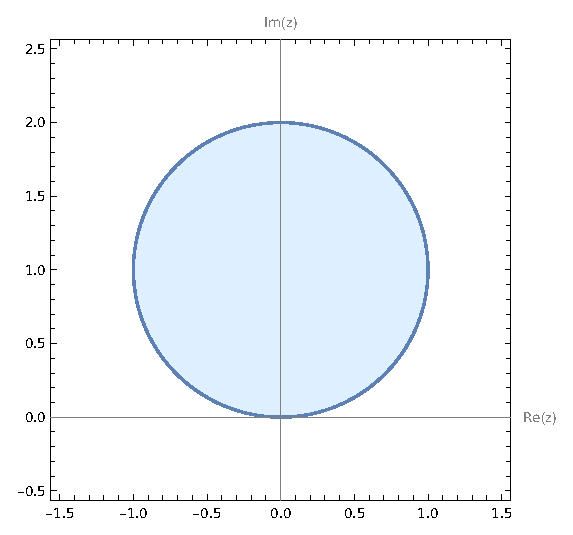
\includegraphics[scale=0.8]{R1.eps}
         \end{figure} 

         En este caso es claro que eso era  una bola.

        \item $|z - 1| > |z - 3|$.\\

        Para este caso primero debemos hacer unas cuentas, note que se puede reescribir la desigualdad como $(z-1)(z-1)>(z-3)(z-3)$, haciendo cositas se llega a que

        $$|z|^2-2 \Re(z)+1^2>|z|^2-6 \Re(z)+9 $$

        de esto se sigue que la región es el semiplano $\Re(z)>2$

         \begin{figure}[H]
         \centering
         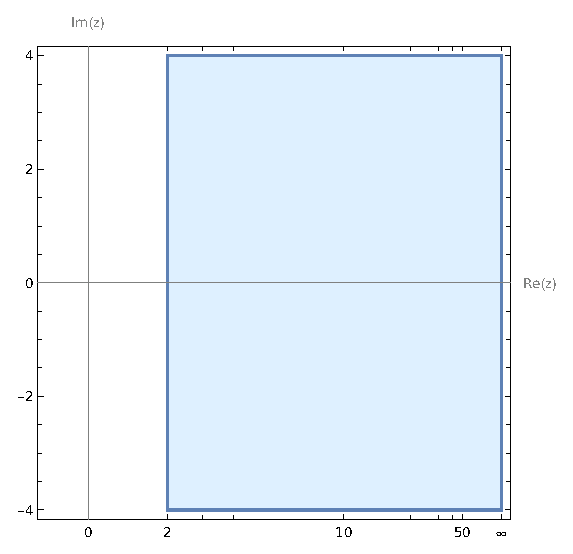
\includegraphics[scale=0.8]{R2.eps}
         \end{figure} 

        \item $\dfrac{1}{z} = \overline{z}$.\\

        Este se hizo en clase, usted llega y dice $z \overline{z}=1=|z|$ y fecho, eso le da el círculo unitario\\

         \begin{figure}[H]
         \centering
         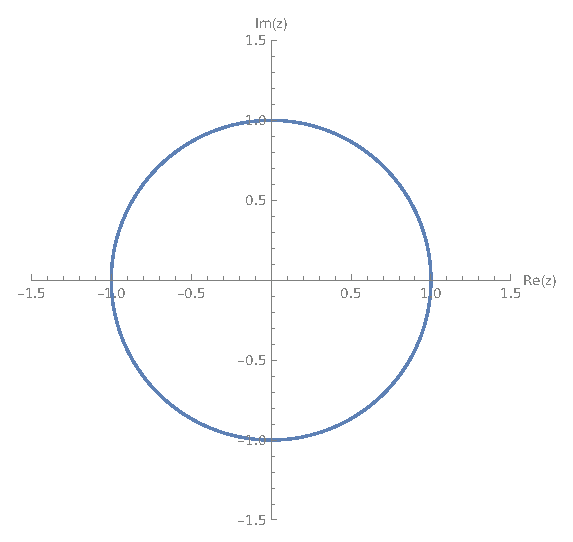
\includegraphics[scale=0.8]{R3.eps}
         \end{figure}

        \item $|z^2 - 1| < 1$.\\

        Esta es coya porque toca saber parametrizar una vaina que no me acuerdo cómo se llama pero el Sergio me dijo el nombre xd


         \begin{figure}[H]
         \centering
         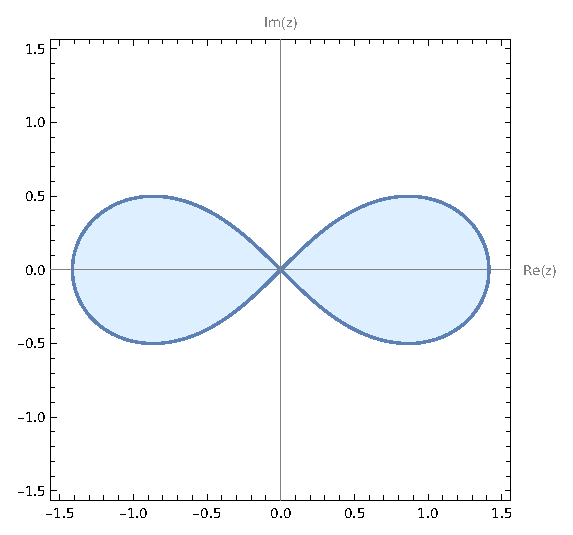
\includegraphics[scale=0.8]{R4.eps}
         \end{figure}

        \item $\left| \dfrac{z - 1}{z + 1} \right| = 1$.\\

        Este caso es fácil porque uno llega y se da cuenta que $|z-1|=|z-(-1)|$, esto dice que la distancia al $1$ y al $-1$ debe ser igual, eso solo nos deja el caso $\Re(z)=0$, los complejos en esa recta vertical por simetría.\\

        \begin{figure}[H]
         \centering
         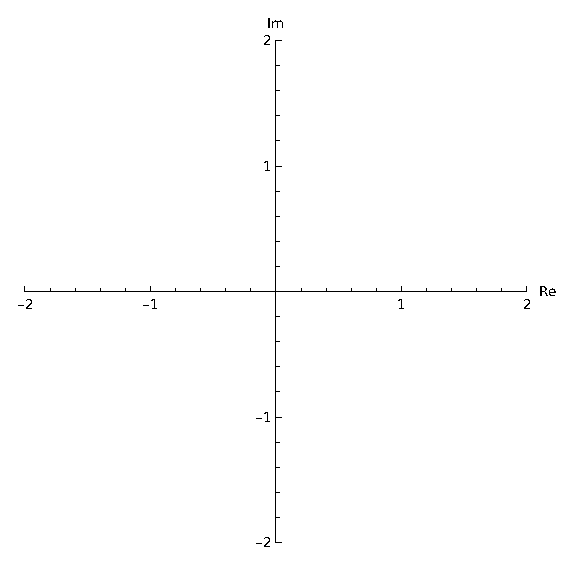
\includegraphics[scale=0.8]{R5.eps}
         \end{figure}

        Ahí medio se ve la verdad... Además imaginese que eso va de $-\infty$ a $\infty$ porque no supe programar eso.
        \item $|z|^2 = \operatorname{Im}(z)$.\\

        Esta anda  coya y toca  preguntarle a Cesar, en especial porque no sabemos cómo dibujar eso. Con Sergio hicimos esto, sea $z=a+bi$, entonces nos queda

        $$|z|^2 =a^2+b^2=b.$$

        Si usted usa la chicharronera le queda que

        $$ b =\frac{1 \pm \sqrt{2-4 a^2}}{2},$$

        y ahí ya se putea la cosa
    \end{enumerate}

    \item \textbf{Definición 1}: Un conjunto se dice conexo si dados dos puntos diferentes en el conjunto, estos se pueden unir por una poligonal (formada por un número finito de segmentos rectos) contenida en el conjunto. Si además el conjunto es abierto, se le llama entonces \textit{Dominio}.

    \textbf{Definición 2}: Un punto $w \in S \subset \mathbb{C}$, se dice es de acumulación si todo $D(w; r) \setminus \{w\}$, $r > 0$ contiene al menos un punto de $S$ (en particular, contiene infinitos puntos de $S$). Clasifique los conjuntos siguientes según sean abiertos, cerrados, acotados, conexos, dominios; encontrar además sus puntos de acumulación y de adherencia.
    \begin{enumerate}
        \item $|z - 1| < 1$.

        

        \item $|\operatorname{Im}(z)| < 3$.
        


        \item $|z + i| + |z - i| = 1$.



        \item $0 < |z| < 2$.
        


        \item $0 < \arg(z) < \frac{\pi}{6}$.
        


        \item $\operatorname{Re}(z^2) \geq 0$.
        


        \item $\operatorname{Re}(z - i \overline{z}) \geq 0$.
    \end{enumerate}
\end{enumerate}

\end{document}